\documentclass{standalone}
\usepackage{pgfplots}
\pgfplotsset{compat=1.18}
\begin{document}
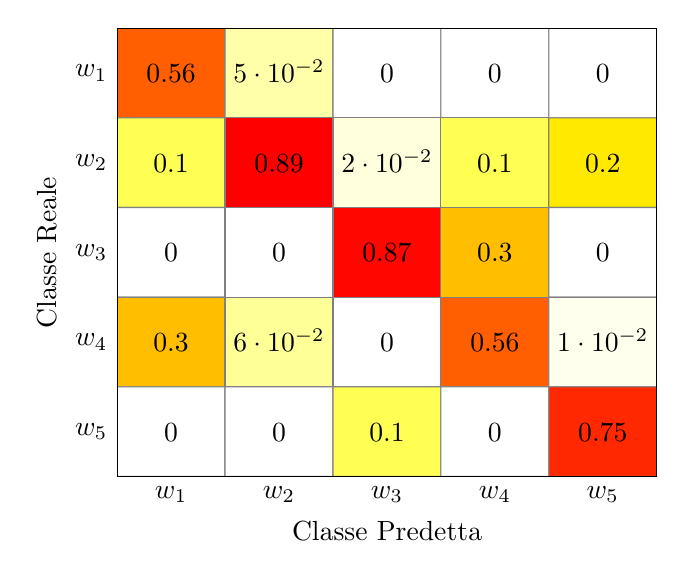
\begin{tikzpicture}
    \begin{axis}[
            colormap={hot}{color(0cm)=(white); color(0.5cm)=(yellow); color(1.5cm)=(orange); color(3cm)=(red)},
            xlabel={Classe Predetta},
            ylabel={Classe Reale},
            xticklabels={$w_1$, $w_2$, $w_3$, $w_4$, $w_5$}, % changed
            xtick={0,...,4}, % changed
            xtick style={draw=none},
            yticklabels={$w_1$, $w_2$, $w_3$, $w_4$, $w_5$}, % changed
            ytick={0,...,4}, % changed
            ytick style={draw=none},
            enlargelimits=false,
            nodes near coords={\pgfmathprintnumber\pgfplotspointmeta},
            nodes near coords style={
                yshift=-7pt
            },
        ]
        \addplot[
            matrix plot,
            mesh/cols=5, % changed
            point meta=explicit,draw=gray
        ] table [meta=C] {
            x y C
            0 0 0.56
            1 0 0.05
            2 0 0
            3 0 0
            4 0 0
            
            0 1 0.1
            1 1 0.89
            2 1 0.02
            3 1 0.1
            4 1 0.2
            
            0 2 0
            1 2 0
            2 2 0.87
            3 2 0.3
            4 2 0
    
            0 3 0.3
            1 3 0.06
            2 3 0
            3 3 0.56
            4 3 0.01
    
            0 4 0
            1 4 0
            2 4 0.1
            3 4 0
            4 4 0.75
            
        }; % added every entry where x=4 or y=4
    \end{axis}
\end{tikzpicture}
\end{document}